\documentclass[openright, a4paper]{article}
\usepackage{graphicx}
\usepackage{kotex}
\usepackage{minted}
\usepackage{setspace}
\usepackage{underscore}
\usepackage{caption}
\usepackage[margin=3cm]{geometry}
\newcommand{\code}[1]{\texttt{#1}}
\setminted{
    linenos=true,
    autogobble,
}
\newenvironment{longlisting}{\captionsetup{type=listing}}{}
\captionsetup{labelformat=empty,labelsep=none}

\title{2024학년도 컴퓨터구조 Lab Assignment \#5\\
        Cache}

\author{김도영, 선민수}
\date{2024년 5월 29일}

\onehalfspacing
\begin{document}

\maketitle

%%%%%%%%%%%%%%%%%%%%%%%%%%%%%%%%%%%%%%%%%%%%%%%%%%%%%
%                   Introduction                    %
%%%%%%%%%%%%%%%%%%%%%%%%%%%%%%%%%%%%%%%%%%%%%%%%%%%%%

\section{Introduction}
이 과제에서는 Lab Assignment \#4에서 구현했던 Pipelined CPU에 더해, 주 메모리의
값을 임시로 저장하는 

\begin{itemize}
    \item Multi-Cycle CPU에서는 Branch의 Taken/Not Taken이 결정된 이후 다음 Instruction이 Fetch된다. 반대로 Pipelined CPU는 Multi-Cycle CPU와 달리 Branch의 Taken/Not Taken이 결정되기 전에 다음 Instruction이 Fetch된다.
    \item Multi-Cycle CPU는 언제나 Branch의 결과에 맞추어 다음 Instruction을 Fetch하지만, Pipelined CPU의 경우 Branch Instruction 직후 Fetch된 Instruction이 Branch Not Taken일 경우 유효하지만, Taken일 경우 유효하지 않아 Stall을 발생시킨다.
\end{itemize}

위와 같은 이유로 Pipelined CPU에서는 Branch Instruction 직후 Fetch되는 Instruction의 위치가 중요하다. Pipelined CPU는 이를 Branch Prediction을 통해 해결하며, Branch Prediction의 전략은 다양하다. 본 과제에서는 2-Bit Saturation Counter를 응용한 2-Bit Global Branch Prediction 전략을 사용하여 구현한다.

%%%%%%%%%%%%%%%%%%%%%%%%%%%%%%%%%%%%%%%%%%%%%%%%%%%%%
%                      Design                       %
%%%%%%%%%%%%%%%%%%%%%%%%%%%%%%%%%%%%%%%%%%%%%%%%%%%%%

\section{Design}
본 과제에서 구현한 Pipelined CPU에서의 Control Flow Data Path는 교과서의 강의 교안을 기준으로 구현하였으며, Branch Prediction은 2-bit Saturation Branch Prediction을 적용하여 구현하였다.

\hfill

Pipelined CPU는 이전 Multi Cycle CPU와 같이 IF - ID - EX - MEM - WB의 스테이지로 나뉘어서 실행된다. Multi Cycle CPU와의 차이점은 모든 스테이지가 동시에 사용된다는 점으로, Instruction 1이 ID 스테이지에서 처리될 때, 다른 Instruction 2는 IF 스테이지를 거치는 식으로 동시에 최대 5개의 instruction을 처리한다.

\hfill

Data hazard가 발생하는 경우에는 Hazard Detection Module을 통해서 Hazard 발생을 탐지하고 Hazard가 발생된 원인(레지스터의 WB Stage, Store Instruction의 MEM Stage 등)이 모두 완료될 때까지 Stall하여 이를 해결한다.

\hfill

레지스터가 아직 WB되지 않아 발생하는 Hazard는 Data Forwarding을 통하여 WB 이전에 값을 받아와 Stall되는 시간을 줄여, 최적화할 수 있다. 해당 과제에서는 Data Forwarding을 함께 구현한다.

\hfill

구현한 Pipelined CPU는 아래와 같은 구조를 가진다. (단, 그림에서 Data Forwarding Unit과 Hazard Detection Module은 표현되지 않았다.) 구현에서의 \code{wire}나 \code{reg}의 이름은 아래 그림에서 제시된 이름을 사용한다.

\hfill

%% TODO: SCHEMATIC IMAGE
{
    \begin{figure}[!h]
        \centering
        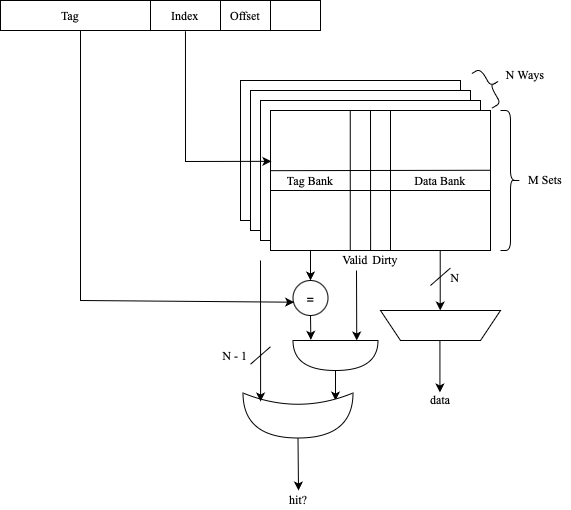
\includegraphics[width=\textwidth]{img/schematic.png}
        \caption{Design of Pipelined CPU}
    \end{figure}
}

\hfill

Pipelined CPU의 Control Flow Data Path에 관여하는 세부 모듈들과 각각의 역할은 아래와 같다.

\hfill

\begin{itemize}
    \item PC: 현재의 program counter 값을 저장하는 모듈로, clock의 positive 
    edge마다 \code{next_pc} 신호를 받아 \code{pc_write} 신호가 \code{1}일 때 
    program counter를 업데이트하는 동기 회로이다.

    \item Hazard Detection Module: 현재 실행되어야 하는 Instruction이 앞서 실행된 Instruction의 실행 종료를 기다려야 하는지에 대한 여부를 판단하는 모듈이다. 주어진 Instruction에 대해 이전 Instruction의 Dependency를 계산하는 비동기 회로이다.

    \item Forwarding Unit: Stall로 인한 딜레이를 최소화하고자 ALU의 피연산자를 MEM 혹은 WB Stage에서 바로 Fetch할 수 있는지에 대한 여부를 판단하여, MEM 혹은 WB Stage에서의 사용때문에 생기는 Stall을 줄일 수 있는 모듈이다. 주어진 Instruction에 대해 해당 피연산자들이 어느 단계에서 사용되고 있는지를 판단하는 비동기 회로이다.
    
    \item Control: 현재 명령어의 opcode를 받아 명령어의 실행 과정에 따라 
    해당하는 control 신호를 계산하는 비동기 회로이다.
    
    \item Registers: CPU의 programmer visible state 중 하나인 레지스터이다. 
    \code{x0}부터 \code{x31}까지 총 32개를 가지고 있다. Register의 업데이트는 clock의 negative 
    edge에서 업데이트되는 동기 회로이며, Register의 읽기의 경우 비동기 회로이다.

    \item Immediate Generator: 명령어를 받아 명령어에 따른 immediate 값을 계산하는 모듈로, 
    비동기 회로이다.

    \item ALU control: ALU가 수행해야 할 연산을 지정해주는 ALU control 신호를 
    계산하는 비동기 회로 모듈이다.

    \item ALU: 두 입력값과 ALU contorl 신호를 받아 해당하는 연산을 하는 
    모듈로, 입력이 바뀌면 출력도 곧바로 바뀌는 비동기 회로이다.

    \item Memory: 실제 CPU에 연결된 memory의 역할을 하는 모듈로, Instruction Memory와 Data Memory를 구분하여 사용한다. clock의 positive edge마다 입력에 따라 메모리 값을 변경하는 동기 회로이다.

    \item Pipeline Register: 각 Stage 별로 다음 Stage에 넘겨주어야 할 Control Signal이나 Register의 정보 등의 신호를 저장하는 Register이다. 스테이지의 사이마다 존재하여 값을 넘겨준다. Clock의 Positive Edge마다 Stage에서 계산된 결과를 Fetch하여 Register의 값을 변경하는 동기 회로이다.
\end{itemize}

%%%%%%%%%%%%%%%%%%%%%%%%%%%%%%%%%%%%%%%%%%%%%%%%%%%%%
%                 Implementation                    %
%%%%%%%%%%%%%%%%%%%%%%%%%%%%%%%%%%%%%%%%%%%%%%%%%%%%%

\section{Implementation}

아래 명시되지 않은 모듈은 기존 4-1의 내용과 동일하다. \\

\subsection{Branch Predictor}

\begin{longlisting}
    \begin{minted}[fontsize=\footnotesize]{Verilog}
  always @(posedge clk) begin
    if(reset) begin
      for(i = 0; i < ENTRY_NUMBER; i = i + 1) begin
        branch_target_buffer[i] <= 0;
        pattern_history_table[i] <= `BP_SN;
        tag_table[i] <= 0;
      end
    end else if(is_control_flow && is_exist) begin
      branch_target_buffer[idx_to_update] <= branch_target;
      
      case(pattern_history_table[idx_to_update])
      `BP_ST:
        pattern_history_table[idx_to_update] <= (is_correct ? `BP_ST : `BP_WT);
      `BP_WT: 
        pattern_history_table[idx_to_update] <= (is_correct ? `BP_ST : `BP_WN);
      `BP_WN: 
        pattern_history_table[idx_to_update] <= (is_correct ? `BP_SN : `BP_WT);
      `BP_SN: 
        pattern_history_table[idx_to_update] <= (is_correct ? `BP_SN : `BP_WN);
      default:
        pattern_history_table[idx_to_update] <= `BP_SN;
      endcase
    end else if(is_control_flow && !is_exist) begin
      branch_target_buffer[idx_to_update] <= branch_target;
      tag_table[idx_to_update] <= new_tag;
      pattern_history_table[idx_to_update] <= `BP_SN;
    end
  end

  wire [INDEX_LENGTH - 1: 0] index = current_pc[INDEX_LENGTH + 1: 2];
  wire [TAG_LENGTH - 1: 0] tag = current_pc[31: 32 - TAG_LENGTH];
  wire is_match = (tag_table[index] == tag);
  wire is_taken = pattern_history_table[index][1];

  assign prediction = is_match && is_taken;
  assign predicted_pc = 
    prediction ? branch_target_buffer[index] : (current_pc + 4);
    \end{minted}
    \caption{BranchPredict.v}
\end{longlisting}

본 과제에서 구현한 Branch Predictor는 2-Bit Saturation Counter를 기반으로 한 Global Branch Predictor이다.
32 Entry를 가지는 PHT와 BTB를 이용하여 구현하였으며, clk 신호에 맞추어 업데이트되는 Synchronous 모듈이다. \\

\subsection{Branch Pre-Fetch}

\begin{longlisting}
    \begin{minted}[fontsize=\footnotesize]{Verilog}
always @(*) begin
    case(btype)
        `FUNCT3_BEQ: bcond = (rs1_dout == rs2_dout);
        `FUNCT3_BNE: bcond = (rs1_dout != rs2_dout);
        `FUNCT3_BLT: bcond = (rs1_dout  < rs2_dout);
        `FUNCT3_BGE: bcond = (rs1_dout >= rs2_dout);
        default: bcond = 0;
    endcase
end
    \end{minted}
    \caption{BranchPreFetcher.v}
\end{longlisting}

Branch Pre-Fetch 모듈은 기존의 Pipelined CPU에서 Branch Condition을 계산하는 부분을 MEM Stage에서 ID Stage로 옮겨온 모듈이다.
기존의 Branch Condition 계산과 동일한 메커니즘이 사용되며, Asynchronous한 모듈이다. \\

\subsection{PC Generator}

\begin{longlisting}
    \begin{minted}[fontsize=\footnotesize]{Verilog}
assign next_pc = PC + shifted_imm;
assign shifted_imm = imm << 2;
    \end{minted}
    \caption{PCGenerator.v}
\end{longlisting}

기존 4-1에서 구현하였던 Pipelined CPU에서는 immediate 값과 Program Counter 값을 합산해주는 모듈이 구현되지 않았다.
기존의 Schematic에서는 해당 모듈이 EX Stage에 존재하였으나 ID Stage로 옮겨서 구현하였으며, Asynchronous한 모듈이다. \\

\subsection{Control Unit}

\begin{longlisting}
    \begin{minted}[fontsize=\footnotesize]{Verilog}
    wire [6:0] opcode = inst[6:0];

    wire is_arith = (opcode == `ARITHMETIC);
    wire is_arith_imm = (opcode == `ARITHMETIC_IMM);
    wire is_load = (opcode == `LOAD);
    wire is_store = (opcode == `STORE);

    assign reg_write = !is_store && !is_branch;
    assign alu_src = !is_arith && !is_branch;
    assign mem_read = is_load;
    assign mem_write = is_store;
    assign mem_to_reg = is_load;
    assign pc_to_reg = is_jal || is_jalr;
    assign alu_op[0] = 1'b0;
    assign alu_op[1] = !is_load && !is_store && !is_jalr;
    assign is_jalr = (opcode == `JALR);
    assign is_jal = (opcode == `JAL);
    assign is_branch = (opcode == `BRANCH);
    assign is_ecall = (opcode == `ECALL);
    \end{minted}
    \caption{ControlUnit.v}
\end{longlisting}

Control Unit은 주어진 instruction에서 opcode에 따라 필요한 Control Value를 계산하여 산출하는 Asynchronous 모듈이다. \\

\subsection{Hazard Detection Module}

\begin{longlisting}
\begin{minted}[fontsize=\footnotesize]{Verilog}
  wire is_arith = (ID_opcode == `ARITHMETIC);
  wire is_store = (ID_opcode == `STORE);
  wire is_branch = (ID_opcode == `BRANCH);
  wire is_lui = (ID_opcode == `LUI);
  wire is_auipc = (ID_opcode == `AUIPC);
  wire is_jal = (ID_opcode == `JAL);
  wire is_jalr = (ID_opcode == `JALR);
  wire is_rs1_zero = (ID_rs1 == 5'b0);
  wire is_rs2_zero = (ID_rs2 == 5'b0);

  wire use_rs1 = (!is_lui || !is_auipc || !is_jal) && !is_rs1_zero;
  wire use_rs2 = (is_arith || is_store || is_branch) && !is_rs2_zero;

  wire is_data_hazard_from_EX = 
    ((ID_rs1 == EX_rd) && use_rs1 || (ID_rs2 == EX_rd) && use_rs2) 
      && EX_mem_read;

  wire is_data_hazard_from_MEM = 
    ((ID_rs1 == MEM_rd) && use_rs1 || (ID_rs2 == MEM_rd) && use_rs2)
      && MEM_mem_read;
  
  assign is_data_hazard = is_data_hazard_from_EX || is_data_hazard_from_MEM;
  assign is_control_hazard = 
    (prediction ^ (is_jalr || is_jal || (is_branch && bcond)));
\end{minted}
\caption{HazardDetection.v}
\end{longlisting}

Hazard Detection Module은 현재 Hazard가 발생되어 현재 Pipeline에서의 stall을 발생시켜야 하는지 여부에 대해 판단하는 모듈이다.
주어진 Instruction과 사용되는 레지스터, Branch Predictor의 Prediction을 이용하여 Hazard를 판단하고 이를 출력하는 비동기 회로이다. \\

\subsection{Forwarding Unit}

\begin{longlisting}
    \begin{minted}[fontsize=\footnotesize]{Verilog}
  always @(*) begin
    if((ID_rs1 != 0) && (ID_rs1 == EX_rd) && EX_reg_write)
      forward_1 = 2'b11;
    else if((ID_rs1 != 0) && (ID_rs1 == MEM_rd) && MEM_reg_write)
      forward_1 = 2'b10;
    else if((ID_rs1 != 0) && (ID_rs1 == WB_rd) && WB_reg_write)
      forward_1 = 2'b01;
    else
      forward_1 = 2'b00;

    if((ID_rs2 != 0) && (ID_rs2 == EX_rd) && EX_reg_write)
      forward_2 = 2'b11;
    else if((ID_rs2 != 0) && (ID_rs2 == MEM_rd) && MEM_reg_write)
      forward_2 = 2'b10;
    else if((ID_rs2 != 0) && (ID_rs2 == WB_rd) && WB_reg_write)
      forward_2 = 2'b01;
    else
      forward_2 = 2'b00;
  end
    \end{minted}
    \caption{ForwardingUnit.v}
\end{longlisting}

Forwarding Unit은 현재 ALU에서 사용되어야할 피연산자들이 앞선 EX, MEM, WB Stage 등에서 사용되어 있는지를 판단하고 사용할 수 있을 경우 사전 정의된 \code{forward_1}, \code{forward_2}를 통해서 알리는 모듈이다.
주어진 Instruction을 이용하여 Signal을 생성하는 Asynchronous 모듈로 구현하였다. \\

\subsection{CPU}

(아래는 CPU Module의 구현으로, 위에서 설명된 Module의 선언에 대해서는 생략한다.)

\begin{longlisting}
    \begin{minted}[fontsize=\footnotesize]{Verilog}
  // IF stage combinational logics
  assign IF_next_pc = ID_is_correct ? IF_predicted_pc : ID_next_pc;
  assign IF_pc_write = !IF_is_stall;
  assign IF_is_stall = ID_is_data_hazard || (ID_is_jalr && !ID_EX_is_jalr);
  assign IF_is_flush = ID_is_control_hazard;

  // IF/ID stage pipeline register updates
  // IF_is_flush must passed until ID stage, and if current instruction in 
  // ID stage's is_flush is asserted, its mem_write and reg_write must be 
  // de-asserted.
  always @(posedge clk) begin
    if(!IF_is_stall) begin
      IF_ID_is_flush <= reset ? 0 : IF_is_flush;
      IF_ID_prediction <= reset ? 0 : IF_prediction;
      IF_ID_current_pc <= reset ? 0 : IF_current_pc;
      IF_ID_predicted_pc <= reset ? 0 : IF_predicted_pc;
      IF_ID_inst <= reset ? 0 : IF_inst;
    end
  end
  
  // ID stage combinational logics
  assign ID_is_stall = ID_is_data_hazard || (ID_is_jalr && !ID_EX_is_jalr);
  assign ID_is_taken = ID_is_jal || ID_is_jalr || ID_is_branch && ID_bcond; 
  assign ID_rs1 = ID_is_ecall ? 17 : IF_ID_inst[19:15];
  assign ID_branch_target = IF_ID_current_pc + ID_imm; 
  assign ID_is_correct = !(IF_ID_prediction ^ ID_is_taken);

  always @(*) begin
    if(ID_EX_is_jalr)
      ID_next_pc = EX_alu_result;
    else if(ID_is_jal || ID_is_branch && ID_bcond)
      ID_next_pc = ID_branch_target;
    else
      ID_next_pc = IF_ID_current_pc + 4;
  end

  always @(*) begin
    case(ID_forward_1)
    2'b00: ID_rs1_dout = ID_rs1_dout_rf;
    2'b01: ID_rs1_dout = WB_din;
    2'b10: ID_rs1_dout =
      EX_MEM_pc_to_reg ? EX_MEM_current_pc + 4 : EX_MEM_alu_result;
    2'b11: ID_rs1_dout = 
      ID_EX_pc_to_reg ? ID_EX_current_pc + 4 : EX_alu_result;
    default: ID_rs1_dout = 0;
    endcase

    case(ID_forward_2)
    2'b00: ID_rs2_dout = ID_rs2_dout_rf;
    2'b01: ID_rs2_dout = WB_din;
    2'b10: ID_rs2_dout = 
      EX_MEM_pc_to_reg ? EX_MEM_current_pc + 4 : EX_MEM_alu_result;
    2'b11: ID_rs2_dout = 
      ID_EX_pc_to_reg ? ID_EX_current_pc + 4 : EX_alu_result;
    default: ID_rs2_dout = 0;
    endcase
  end

  // ID/EX stage pipeline register updates
  always @(posedge clk) begin
    ID_EX_alu_src <= reset ? 0 : ID_alu_src;
    ID_EX_alu_op <= reset ? 0 : ID_alu_op;
    ID_EX_mem_read <= reset ? 0 : ID_mem_read;
    ID_EX_mem_write <= 
      (reset || IF_ID_is_flush || ID_is_stall) ? 0 : ID_mem_write;
    ID_EX_is_jalr <= reset ? 0 : ID_is_jalr;
    ID_EX_is_jal <= reset ? 0 : ID_is_jal;
    ID_EX_is_branch <= reset ? 0 : ID_is_branch;
    ID_EX_is_correct <= reset ? 0 : ID_is_correct;
    ID_EX_is_halted <= reset ? 0 : ID_is_ecall && (ID_rs1_dout == 10);
    ID_EX_reg_write <= 
      (reset || IF_ID_is_flush || ID_is_stall) ? 0 : ID_reg_write;
    ID_EX_mem_to_reg <= reset ? 0 : ID_mem_to_reg;
    ID_EX_pc_to_reg <= reset ? 0 : ID_pc_to_reg;
    ID_EX_inst <= reset ? 0 : IF_ID_inst;
    ID_EX_current_pc <= reset ? 0 : IF_ID_current_pc;
    ID_EX_branch_target <= reset ? 0 : ID_branch_target;
    ID_EX_rs1_dout <= reset ? 0 : ID_rs1_dout;
    ID_EX_rs2_dout <= reset ? 0 : ID_rs2_dout;
    ID_EX_imm <= reset ? 0 : ID_imm;
  end

  // EX stage combinational logics
  assign EX_alu_in_2 = ID_EX_alu_src ? ID_EX_imm : ID_EX_rs2_dout; 

  // EX/MEM stage pipeline register updates
  always @(posedge clk) begin
    EX_MEM_is_jal <= reset ? 0 : ID_EX_is_jal;
    EX_MEM_is_jalr <= reset ? 0 : ID_EX_is_jalr;
    EX_MEM_mem_read <= reset ? 0 : ID_EX_mem_read;
    EX_MEM_mem_write <= reset ? 0 : ID_EX_mem_write;
    EX_MEM_reg_write <= reset ? 0 : ID_EX_reg_write;
    EX_MEM_mem_to_reg <= reset ? 0 : ID_EX_mem_to_reg;
    EX_MEM_pc_to_reg <= reset ? 0 : ID_EX_pc_to_reg;
    EX_MEM_is_halted <= reset ? 0 : ID_EX_is_halted;
    EX_MEM_inst <= reset ? 0 : ID_EX_inst;
    EX_MEM_rs2_dout <= reset ? 0 : ID_EX_rs2_dout;
    EX_MEM_current_pc <= reset ? 0 : ID_EX_current_pc;
    EX_MEM_alu_result <= reset ? 0 : EX_alu_result;
  end

  // MEM/WB stage pipeline register declarations
  always @(posedge clk) begin
    MEM_WB_is_jal <= reset ? 0 : EX_MEM_is_jal;
    MEM_WB_is_jalr <= reset ? 0 : EX_MEM_is_jalr;
    MEM_WB_reg_write <= reset ? 0 : EX_MEM_reg_write;
    MEM_WB_mem_to_reg <= reset ? 0 : EX_MEM_mem_to_reg;
    MEM_WB_pc_to_reg <= reset ? 0 : EX_MEM_pc_to_reg;
    MEM_WB_is_halted <= reset ? 0 : EX_MEM_is_halted;
    MEM_WB_inst <= reset ? 0 : EX_MEM_inst;
    MEM_WB_dout <= reset ? 0 : MEM_dout;
    MEM_WB_alu_result <= reset ? 0 : EX_MEM_alu_result;
    MEM_WB_current_pc <= reset ? 0 : EX_MEM_current_pc;
  end

  // WB combinational logics
  always @(*) begin
    if(MEM_WB_pc_to_reg)
      WB_din = MEM_WB_current_pc + 4;
    else if(MEM_WB_mem_to_reg)
      WB_din = MEM_WB_dout;
    else
      WB_din = MEM_WB_alu_result;
  end

  // WB sequential logics
  always @(posedge clk) begin
    is_halted <= reset ? 0 : MEM_WB_is_halted;
  end
    \end{minted}
    \caption{cpu.v}
\end{longlisting}

CPU 모듈은 위 Design에서 제시한 대로 다른 모듈 간의 Wiring을 진행하며, 각 Stage별 Pipeline Register의 업데이트를 구현한다. 구현에서 사용된 각 wire와 reg의 이름은 아래의 Convention을 따른다.

\begin{itemize}
    \item Pipeline Register: \code{<FIRST_STAGE_NAME>_<SECOND_STAGE_NAME>_<REGISTER_OR_WIRE_NAME>}
    \item Stage Register: \code{<STAGE_NAME>_<REGISTER_OR_WIRE_NAME>}
\end{itemize}

ECALL에 따라서 종료될 수 있도록 ECALL을 한 후 x17 레지스터의 값 비교를 통해 \code{is_halted}로 데이터를 생성해 Pipelining을 하도록 구현하였다. Pipelining에 의해서 ECALL 이전의 Instruction이 모두 실행 완료되어야 하므로, \code[is_halted] 또한 Stage를 모두 거쳐서 마지막 WB 이후 종료될 수 있도록 구현하였다.

%%%%%%%%%%%%%%%%%%%%%%%%%%%%%%%%%%%%%%%%%%%%%%%%%%%%%
%                    Discussion                     %
%%%%%%%%%%%%%%%%%%%%%%%%%%%%%%%%%%%%%%%%%%%%%%%%%%%%%

\section{Discussion}

\subsection{How to Handle Branch Prediction}

가장 기본적인 Branch Prediction은 Always Taken과 Always Not Taken 전략이 있다. 이는 다음과 같은 특성을 가진다.

\begin{itemize}
    \item Always Taken: 프로그램 실행 중 마주치는 모든 Branch Instruction에 대해서 Branch가 Taken이 될 것이라 예상하여 Branch Taken 시의 \code{PC}에 대해서 미리 Instruction을 Fetch한다.
    \item Always Not Taken: 프로그램 실행 중 마주치는 모든 Branch Instruction에 대해서 Branch가 Not Taken이 될 것이라 예상하여 Branch Not Taken 시의 \code{PC}인 \code{PC+4}에 대해서 미리 Instruction을 Fetch한다.
\end{itemize}

가장 기본적인 전략이지만, 특정 경우에 편향하여 예측하기 때문에, 이를 보완하기 위해서 Counter 기반의 전략을 선택하게 된다. Counter 기반의 대표적인 예시는 다음과 같다.

\begin{itemize}
    \item 1-Bit Counter: \code{Predict Take, 1'b1}, \code{Predict Not Take, 1'b0}의 상태를 가지는 Counter 기반의 전략이다.
    \item 2-Bit Counter: \code{Strongly Taken, 1'b11}, \code{Weakly Taken, 1'b10}, \code{Weakly Not Taken, 1'b01}, \code{Strongly Not Taken, 1'b00}의 4가지 상태를 가지는 Counter 기반의 전략이다. 상태의 전환에 따라서 Saturation Counter와 Hysteresis Counter로 나뉜다.
\end{itemize}

Counter에서 사용되는 bit 수에 따라서 Branch Taken/Not Taken Pattern History를 확인할 수 있다. 초반의 Counter 기반 Branch Predictor는 Branch의 위치(Program Counter)마다 해당 Pattern History를 저장하여 예측하는 방법으로 구현되었다.

이에서 발전된 형태인 Global Path History를 적용하여 McFarling이 제시한 Gshare Branch Prediction는 기존의 PHT와 BTB의 원리처럼 각 PC에 해당하는 Pattern History도 저장하지만, 동시에 Global Path를 확인하여 Branch Prediction에 성능적 향상을 가져왔다.

이를 확장하여 2-Level Branch Direction Predictor 형태로 발전시켰는데, BHT(Branch History Table) + PHT(Pattern History Table)을 결합 형태이다. 각각의 BHT와 PHT의 형태가 Global, per-Set, per-Address인지에 따라서 다양한 형태의 Branch Predictor를 구성한다.

\textbf{본 과제에서 우리는 2-Bit Saturation Counter 기반의 Branch Predictor를 사용하여 Branch Prediction을 진행하였다.}

\subsection{2-Bit Saturation Counter Branch Predictor의 구현}

본 과제에서 구현한 2-Bit global branch predictor는 2-Bit Saturation Counter를 기반으로 한다. Branch Prediction에 의한 Counter의 유한 상태 기계의 Diagram은 다음과 같다.

\begin{figure}[h]
    \centering
    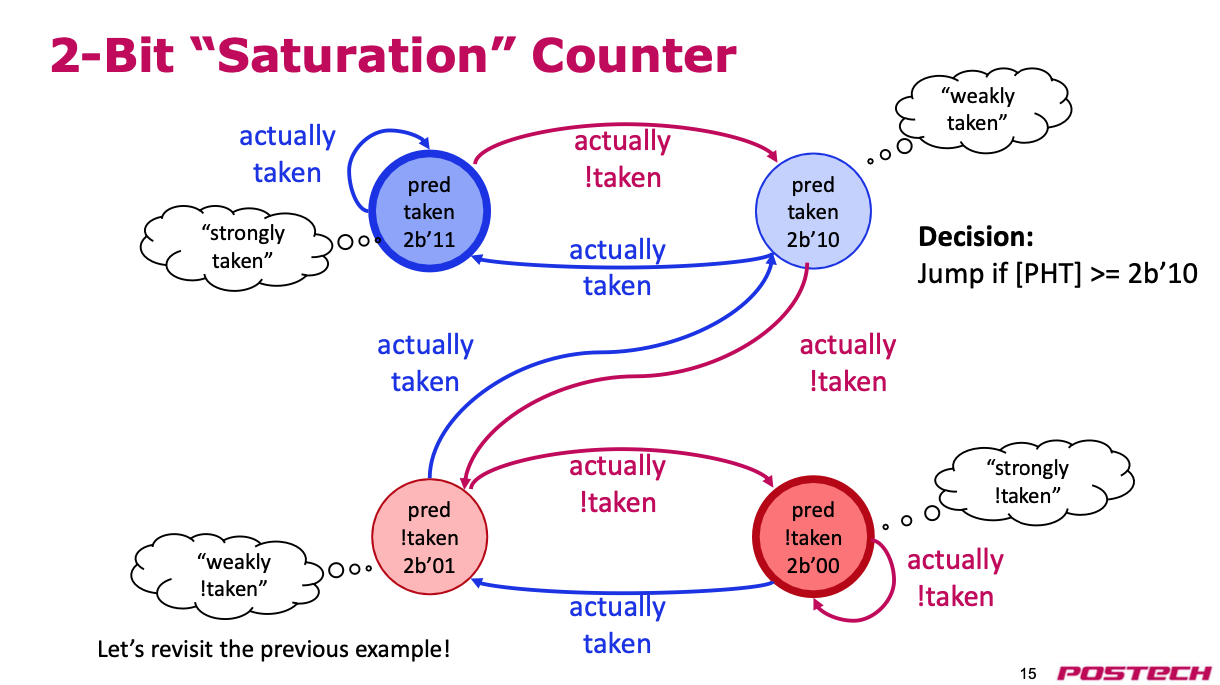
\includegraphics[width=0.8\textwidth]{img/2bit_saturation_counter_FSM_diagram.png}
    \caption{FSM Diagram of 2-Bit Saturation Counter}
\end{figure}

Branch Predictor의 구조는 다음 그림과 같으며, BTB의 index bit는 N=4로 설정되어 전체 32개의 Branch Target Entry를 가지도록 디자인하였다.

\begin{figure}[h]
    \centering
    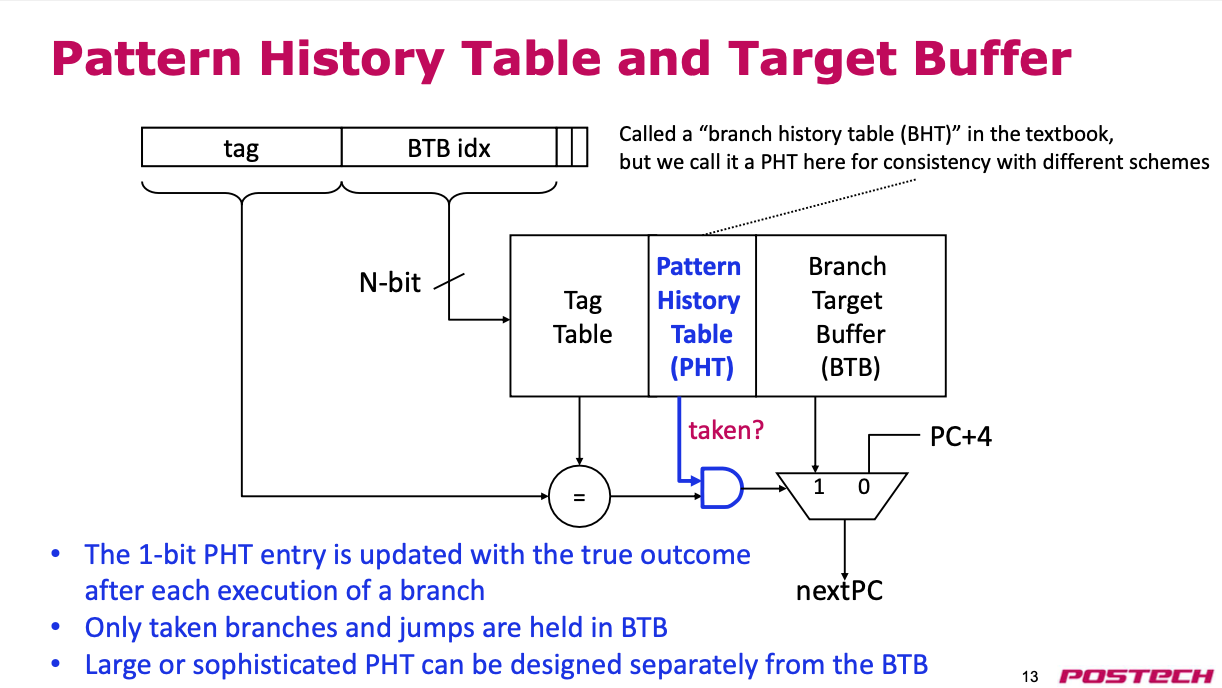
\includegraphics[width=0.8\linewidth]{img/branch_predictor_btb_and_pht.png}
    \caption{Branch Predictor with BTB and PHT}
\end{figure}

2-Bit Saturation Counter는 Strongly Taken, Weakly Taken, Weakly Not Taken, Strongly Not Taken의 4가지 상태로 나타나며, 각 상태에 대한 Predictor의 Prediction과 실제 branch의 taken, not taken에 의한 상태 변화는 아래의 표와 같다.
(실제 코드에서는 Implementation에서 확인할 수 있듯이, \code{BP_ST}, \code{BP_WT}, \code{BP_WN}, \code{BP_SN}으로 각 상태를 나타낸다.)

\begin{table*}[!h]
  \centering
  \begin{tabular}{@{}cccc@{}}
    \hline
     & Prediction & Taken(Real) & Not-Taken(Real) \\
    \hline
    Strongly Taken(2'b11) & Taken & Strongly Taken & Weakly Taken \\
    Weakly Taken(2'b10) & Taken & Strongly Taken & Weakly Not Taken \\
    Weakly Not Taken(2'b01) & Not Taken & Weakly Taken & Strongly Not Taken \\
    Strongly Not Taken(2'b00) & Not Taken & Weakly Not Taken & Strongly Not Taken \\
    \hline
  \end{tabular}
  \caption{Comparison on the Number of Cycles on Different Branch Predictor}
  \label{tab:comparison}
\end{table*}

\subsection{다른 Branch Predictor와의 비교}

다른 방식의 Branch Prediction(Always-Taken, Always-Not-Taken)과 본 과제에서 구현한 2-Bit Saturation Counter Branch Prediction 성능을 비교한 결과는 아래와 같다.

\begin{table*}[!h]
  \centering
  \begin{tabular}{@{}cccc@{}}
    \hline
    Input File & Always-Taken & Always-Not-Taken & Saturation Counter \\
    \hline
    basic & 37 & 37 & 37 \\
    non-controlflow & 46 & 46 & 46 \\
    ifelse & 51 & 51 & 51 \\
    loop & 354 & 362 & 357 \\
    recursive & 1153 & 1229 & 1159 \\
    \hline
  \end{tabular}
  \caption{Comparison on the Number of Cycles on Different Branch Predictor}
  \label{tab:comparison}
\end{table*}

\hfill

실험 결과에 따르면, 2-bit Saturation Counter는 Always-Not-Taken 기반 Branch
Prediction에 비해서는 확연히 나은 성능을 보여주나, Always-Taken 기반에 비해서는
구현의 복잡도가 더 높음에도 불구하고, 오히려 실행에 더 많은 사이클이 걸리는
것을 볼 수 있다. 이는 2-bit Saturation Counter의 경우, Always-Taken에 비해 잘못된
예측을 바로잡기 위해 한 번 더 해당 분기에 들어가 Pattern History Table을 수정하는
과정이 필요해서이다. 따라서, 만약 같은 분기를 더 많이 방문하며, 해당 분기의 실제
방향이 가끔씩 변하는 프로그램이라면, 2-bit Saturation Counter가 Always-Not-Taken
기반 Branch Predictor에 비해 실행에 걸리는 사이클 수가 더 적을 것이다.

%%%%%%%%%%%%%%%%%%%%%%%%%%%%%%%%%%%%%%%%%%%%%%%%%%%%%
%                    Conclusion                     %
%%%%%%%%%%%%%%%%%%%%%%%%%%%%%%%%%%%%%%%%%%%%%%%%%%%%%

\section{Conclusion}

이번 과제에서는 지난 4-1에 이어 Pipelined CPU의 Control Flow DataPath를 구현하는 것을 목적으로 하여, Pipelined CPU를 완성하였다.
기존 Multi-Cycle CPU와는 달리 Branch Taken/Not Taken 여부와 Branch Instruction 다음 Fetch하는 Instruction의 위치에 따라서 Stall이 발생할 수 있기 때문에, Branch Prediction이 중요하다.
2-Bit Saturation Counter 기반의 2-Bit Global Branch Predictor를 구현하여 기존 Always-Taken, Always-Not-Taken 전략과의 비교할 수 있었지만, 주어진 프로그램에 의존하는 특성상 정확한 비교를 할 수 없어 기대한 결과를 확인하지 못하였다.
Single-Cycle CPU, Multi-Cycle CPU, Pipelined CPU의 발전 동안 Data Memory 관점에서의 개선은 미비하였는데, Data Memory 접근성을 늘릴 수 있는 Cache의 필요성을 확인할 수 있었다.

\end{document}